\documentclass[10pt,twocolumn]{article} 
\usepackage{simpleConference}
\usepackage{times}
\usepackage{graphicx}
\usepackage{amssymb}
\usepackage{url,hyperref}
\usepackage{enumitem}
\usepackage{amsmath}

\begin{document}

\title{A comparison of iterative optimizers applied to the MNIST dataset}

\author{Suhrid Deshmukh, Ismail Degani\\
\\
6.337 Final Project\\
May, 6th 2017\\
}

\maketitle
\thispagestyle{empty}

\begin{abstract}
   Abstract for algorithms used and performance on the bench mark problem.
\end{abstract}

\section{Introduction}

Machine learning and optimization has found home in some of the most important machine learning(ML) applications. The fields of machine learning and mathematical programming are becoming increasingly intertwined. Optimization problems lie at the heart of most machine learning approaches. Many optimization algorithms that  are applied in machine learning problems converge at different rates. Manu of the learning algorithms also have different memory footprint and different computational complexity. Studying how different optimization algorithms work when applied in ML applications is therefore an interesting field of research.

The work here explores different optimization schemes that are used in training weight matrices in a Neural net that uses logistic regression. The learning problem in neural nets is formulated in terms of the minimization of a loss function. We can combine the weights and the biases in a neural net in the loss function weight vector w. The loss function is then f(w) with w* as its minima. The learning problem in neural nets is basically searching for a weight vector w* such that the value of the loss function f(w) is minimum at w*. This means that if we evaluate the value of the gradient of f(w) at w*, the gradient is zero.

The loss function in general is a multi-dimensional nonlinear function. In order to minimize the loss function, typically iterative optimization methods are used. The iterative algorithm calculates the loss at each iteration, the change of loss between two steps is called loss decrement. The training algorithm stops when the specified criteria is met. There are multiple training algorithms that are available to train a neural net. We consider three  different algorithms to train a neural net; Gradient descent, Quasi Newton (BFGS),Adam-Optimizer.

The algorithms mentioned above are applied on a simple problem first to make sure that they are functioning properly. They are then used on a benchmark problem which is the classification of handwritten digits in a MNIST data set using a neural net that uses logistic regression. The next section describes each of the algorithms in detail along with the pseudocode and their performance characteristics. 

\section{Algorithms}

\subsection{Gradient Descent}
	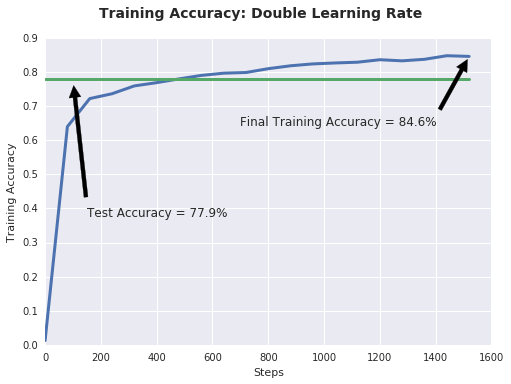
\includegraphics[width=3.5in]{plot1-GradDescent.png}

Gradient descent method is a way to find a local minimum of a function. The way it works is it starts with an initial guess of the solution and then it takes the gradient of the function at that point. We step the solution in the negative direction of the gradient and we repeat the process. The algorithm will eventually converge where the gradient is zero (which correspond to a local minimum). Gradient descent algorithm requires us to choose a learning rate, but it works well to solve the normal equation even when the system is very large. Direct methods might take a long time to solve for the solution, but iterative methods like gradient descent, combined with line search can reach the solution in very few iterations. 

Gradient descent is based on the idea that for a multi-dimensional function, if the derivative exists in the neighborhood of a point, then the function decreases the fastest in the negative direction of the gradient of the function  at that point. This results in the algorithm starting from an initial guess and then repeatedly calculating the gradient at the new guess and moving in the direction opposite to that gradient. The next section describes the pseudocode for gradient descent. 

\subsubsection{Gradient Descent Pseudocode}

\textbf{Inputs:} $(P,V,\eta,\epsilon)$ where P is the parameter space, $V:P \rightarrow R$ is the objective function, $\eta$ is the step size, and $\epsilon$ is the tolerance for the stopping threshold. \\
\textbf{Output:} A point $p^*\in P$ that approximates the minimum of the function V.\\
\textbf{Process:}\\
\begin{enumerate}
\item Randomly select an initial guess $p_{0}$ in the parameter space P
\item Let $i\leftarrow 0$
\item Repeat until $\delta{V} < \epsilon$
	\begin{enumerate}[label=(\alph*)]
	\item Compute the gradient vector $\nabla{V(p_i)}$ of V at $p_{i}$ if possible or estimate $\nabla{V(p_i)}$ as the direction in which V increases fastest from $p_{i}$
	\item Let $p_{i+1} \leftarrow p_{i} - \eta\nabla{V}$
	\item Let $\delta{V}\leftarrow V(p_i) - V(p_{i+1})$
	\item Let $i \leftarrow i+1$
	\end{enumerate}
\item Output $p_{i}$
\end{enumerate}

\subsection{Adam Optimizer}

The Adam Optimizer [1] is a member of a class of "adaptive" gradient descent optimizers which adjust their learning rate $\alpha$ at each iteration in order to converge more efficiently. This adaptive behavior significantly reduces the impact of a badly chosen initial learning rate $\alpha$, which can be difficult to determine. Adam is specifically optimized for sparse datasets as are many similar algorithms in this class. This makes it an excellent candidate for MNIST data which is monochrome and therefore predominantly zero-value. 

The Adam algorithm stores a history of previous gradients $v_t$ and squared gradients $m_t$, also known as first and second moments. In order to compute the current gradient, Adam applies exponentially decaying factors $ \beta_1$ and $\beta_2$ to the first and second moments. It finally calculates bias-adjusted values of these moments $\hat{v}_t , \hat{m}_t $ , and applies a smoothing term $\epsilon$ which avoids division by zero. Pseudocode is given below:

\subsubsection{Algorithm 1: Adam optimization step}
\begin{enumerate}
\item while  $ f ( \theta_t ) > \tau $ 
	\begin{enumerate}
	\item$ t = t + 1 $
	\item$g_t = \nabla_{\theta} f_t (\theta_{t-1})$
	\item$ m_t = \beta \cdot m_{t-1} + (1-\beta_1) \cdot g_t  $
	\item$ v_t = \beta_2 \cdot v_{t-1} + (1+\beta_2) \cdot g_t^2  $
	\item$\hat{m}_t =\frac{m_t}{1-\beta_1^t}  $
	\item$\hat{v}_t = \frac{v_t}{1-\beta_2^t}  $
	\item$ \theta_t = \theta_{t-1} - \alpha \cdot  \frac{{\hat{m}_t}}{\sqrt{\hat{vt}} + \epsilon} $
	\end{enumerate}
\item end while
\end{enumerate}

\subsection{BFGS}
Some of the optimization algorithms like the Newton's method requires the computation of the Hession or the Jacobian. In case the Hessian or Jacobian is absent or too expensive to calculate, we can resort to quasi-newton methods. Quasi-Newton methods are also used to to calculate the roots of a polynomial or as an optimization algorithm. They are typically used in lieu of Newtons method. This will be the main algorithm that will be explored in detail in this piece of work. The goal of this paper is not to prove that BFGS is the most appropriate algorithms to be used in machine learning problems, but to explore the algorithms on some of the traditional machine learning problems and explore how they perform compared to some competing algorithms. 

BFGS essentially is therefore an approximation to the Newtons method. The main advantage of the BFGS method is that you need not evaluate the Hessian explicitly. Newtons method or BFGS are not guaranteed to converge if the function does not have a quadratic Taylor expansion near the optimal point.


\subsubsection{BFGS pseudocode}
When the objective function is quadratic and of the form $f(w) = \frac{1}{2}w^T Q w + w^T b$, the BFGS method with exact line search is given as follows, given an initial point $w^{(0)}$, an initial estimate of the inverse Hessian $H^{(0)}$, and a stopping threshold $\epsilon$.The pseudocode for BFGS is given below. \\
\begin{enumerate}
\item k = 0
\item $\nabla f^{(0)} = Qw^{(0)} - b$
\item Loop
\begin{enumerate}[label={(\roman*)},leftmargin=2\parindent]
\item $\Delta w^{(k)} = - H^{(k)}\nabla f^{(k)}$
\item $\alpha^{(k)}= -\frac{\Delta (w^{(k)})^T \nabla f^{(k)} }{\Delta (w^{(k)})^T Q \nabla f^{(k)}}$
\item $w^{(k+1)} = w^{(k)} + \alpha^{(k)}\Delta w^{(k)}$
\item $\nabla f^{(k+1)} = Qw^{(k+1)} - b$
\item If $\lVert  \nabla f^{(k+1)} \rVert_{2} \leq \epsilon$ then terminate
\item $s^{(k)} = w^{(k+1)} - w^{(k)}$
\item $y ^{(k)} =  \nabla f^{(k+1)}  -  \nabla f^{(k)} $
\item $\rho^{(k)} = \frac{1}{(y^{(k)})^Ts^{(k)}}$
\item $H^{(k+1)} = (I - \rho^{(k)} s^{(k)}(y^{(k)})^T)H^({k}) (I - \rho^{(k)} y^{(k)}(s^{(k)})^T) +\rho^{(k)} s^{(k)}(s^{(k)})^T $
\item k = k+1
\end{enumerate}
\item return $w^{(k)}$
\end{enumerate}

\section{Benchmark problem description}
Describe your benchmark problems here. Describe the inputs and outputs of the problems such that the reader outside your �field can understand their meanings. If there are numerical challenges associated with these problems, describe them.

There are many traditional ML problems that have been used to test the algorithms on. Modified National institute of standards and technology (MNIST) is one such data set. This is the defacto "hello world" data set for machine learning problems. Since its release in 1999, this classic dataset of handwritten images has served as the basis for benchmarking classification algorithms. As new machine learning techniques emerge, this data set remains a classic dataset to test the techniques on.

MNIST consists of handwritten digits from 0-9 and the problem here is to ask the machine to classify them from 0-9. Typically Neural nets are used to solve this classification problem. As mentioned in the beginning, Neural nets involve an optimization problem that needs to decide the best weights to use in the neural nets. In order to make the data set more manageable for optimization, some preconditioning was done to make the data set suitable for the algorithm to take as input. Some of the preconditioning involves increasing the contrast in the images and  the data set is also down sampled to a 28*28 to reduce the dimensionality of the problem.

MNIST with vizualization
Preconditioning of the data set
Reduce the dimensionality, reduce the greyscale to 0,1
Downsample from 300dpi to 28*28
Some discussion on logistic regression maxes out at 94\% accuracy. Neural nets improve that to 99.8\%. 


\section{Performance Characteristics}

\textbf{Introduce the performance characteristics you are going to measure. If you have theoretical estimates on these performance characteristics, derive them here.}

Some of the performance characteristics that were looked at were the number of flops per iteration of the algorithm and also the time taken in seconds for the algorithm to run until convergence. Comparing the number of flops, theoretical Vs. practical did not make much sense because it was very hardware dependent and some of the packaged implementations were far more optimized that the basic implementations of the otherwise more optimal algorithms. Therefore the trends in the theoretical flops were compared with the trends in time taken for the algorithms to converge. 

The total number of flops per iteration in Gradient descent algorithm for a 2D objective function is derived as follows. The most expensive step in the gradient descent algorithm is the updating step of the solution which is given by 


$mn^2$ flops for Ax = b for MNIST problem 784X10 matrix. 
Iterative algorithms do $n^2$ per iteration

Time per iteration
Time to convergence 
Steps to convergence
Training accuracy and test accuracy 

Toy problem works
MNIST with logistic regression
(MNIST with CNN)
Flops of each algorithm (theoretical )
Calculate the elapsed time (relative measure)


\subsection{Gradient Descent Performance Characteristics}
\subsubsection{Gradient Descent Performance Characteristics Toy Problem}
\subsubsection{Gradient Descent Performance Characteristics MNIST}

\subsection{Adam Optimizer Performance Characteristics}
\subsubsection{Adam Optimizer Performance Characteristics Toy Problem}
\subsubsection{Adam Optimizer Performance Characteristics MNIST}
The following section compares gradient descent, adam, and BFGS optmizers on a linear least squares Ax = b optimization, and a logistic regression to solve the MNIST problem.


\subsection{BFGS Performance Characteristics}
\subsubsection{BFGS Performance Characteristics Toy Problem}
\subsubsection{BFGSPerformance Characteristics MNIST}

\section{Numerical results and discussion}
Report the numerical results generated by yourself for the benchmark problems. Include numerical measurements of the performance characteristics and compare them with theoretical estimates. Discuss the di�erence in these results between the algorithms you tested.
Accuracies on different data sets
Show the python normalized flops plot here
\section{Conclusion}





\bibliographystyle{abbrv}
\bibliography{refs}
\end{document}
